\chapter{Progettazione del tool}

%TODO: dire meglio che fa rate, far mostrare il grafico UML prima mostrandolo a pezzi

% TODO: sistemare UML e mostrare pezzo per pezzo cosa fa

% TODO: citare il paper di libRoadRunner

In Figura \ref{fig:uml} è mostrato il diagramma UML che evidenzia le componenti centrali del tool che si appoggia al framework apricopt.

Apricopt ha delle interfaccie che permettono di modellare problemi di ottimizzazione BlackBox, in particolare quei problemi che richiedono la simulazione di un modello biologico.

Al centro del framework è il BlackBoxSolver, che ha il compito di cercare i parametri ottimali.

Esso è un interfaccia, una classe può essere estesa ad essa per implementare un algoritmo di ottimizzazione, per esempio per quanto riguarda l'algoritmo evolutivo di OpenAI. Oppure si possono usare ottimizzatori terzi come Nevergrad o Nomad.

I problemi black box che stiamo considerando sono la stima dei parametri di un dato modello biologico.

La loss function $\mathcal{L}$ 
può essere passata attraverso 
SimulableBlackBox che simula 
il modello con i parametri 
$ \theta $  e calcola 
$\mathcal{L}(\theta,\mathcal{T}(\theta))$ dove $\mathcal{T}(\theta)$ è la traiettoria del sistema con i parametri $\theta$.

Si può specificare un valore $B$ tale per cui se vengono trovati dei parametri tale che $\mathcal{L}(\theta) \leq B$ allora i parametri sono sufficientemente buoni.

Nell'algoritmo \ref{alg:cap} si può vedere l'implementazione di NevergradSolver.

Per la classe OpenAISolver viene sovrascritto il metodo solve con l'algoritmo \ref{alg:openai_algo} dove i suoi iperparametri vengono
presi dal SolverParameters.


% TODO: descrivere l'interfaccia di Nevergrad
% TODO: spiegare che anche la classe OpenAISolver ha l'algoritmo descritto nel capitolo precedente
% dove prende gli iperparametri da params

\begin{algorithm}
\caption{Metodo solve sovrascritto dalla classe Nevergrad solver}\label{alg:cap}
\begin{algorithmic}[1]
\State \textbf{Input:} problem: BlackBox, params: SolverParameters
\State $\text{optimizer } \gets \text{ algoritmo presente in Nevergrad preso dai params}$
\State $B \gets$ minimo preso dai parametri params
\While{$i \in 1..*$}
    \State $\theta \gets \text{ optimizer.ask()}$
    \State val $\gets$ problem.evaluate($\theta$) 
    \If{val $\leq B$}
        \Return{$\theta$}
    \EndIf
    \State $\text{optimizer.tell}(\theta, val)$
\EndWhile
\end{algorithmic}
\end{algorithm}

% TODO: spiegare l'ordinamento delle specie

\begin{figure}[htbp]
    \centering
    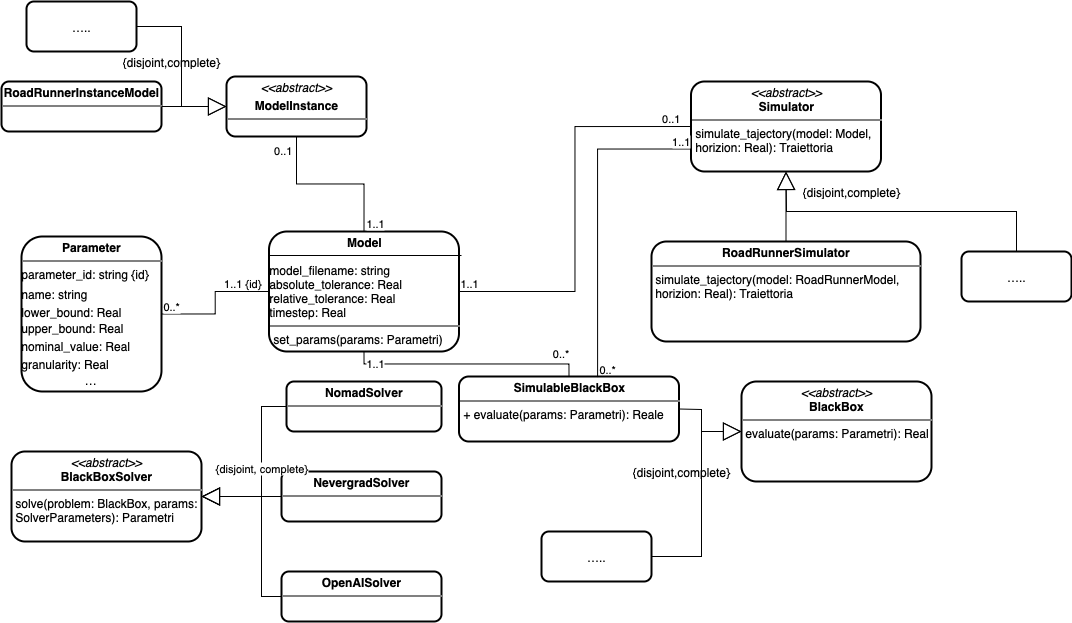
\includegraphics[width=1\textwidth]{analisi.png}%
    \caption{UML}
    \label{fig:uml}
\end{figure}


